\section{Modelo de Banco de Dados}

O modelo de banco de dados do sistema \textbf{Tropical Mix} foi desenvolvido para garantir a integridade, consistência e eficiência no armazenamento e recuperação das informações. A estrutura foi planejada para atender aos requisitos de controle de estoque, registro de vendas e gerenciamento de usuários, assegurando a integridade referencial e o correto relacionamento entre as entidades do sistema.

\subsection{Modelo Conceitual (DER/MER)}

A Figura~\ref{fig:mer-tropicalmix} representa o \textbf{modelo conceitual} do sistema \textbf{Tropical Mix} que foi desenvolvido com o objetivo de representar, de forma abstrata, as principais entidades e relacionamentos do sistema Tropical Mix. Nessa etapa, foram definidas as regras de negócio, cardinalidades e interações entre os elementos do sistema, sem considerar detalhes de implementação física do banco de dados. 
.

\begin{figure}[H]
    \centering
    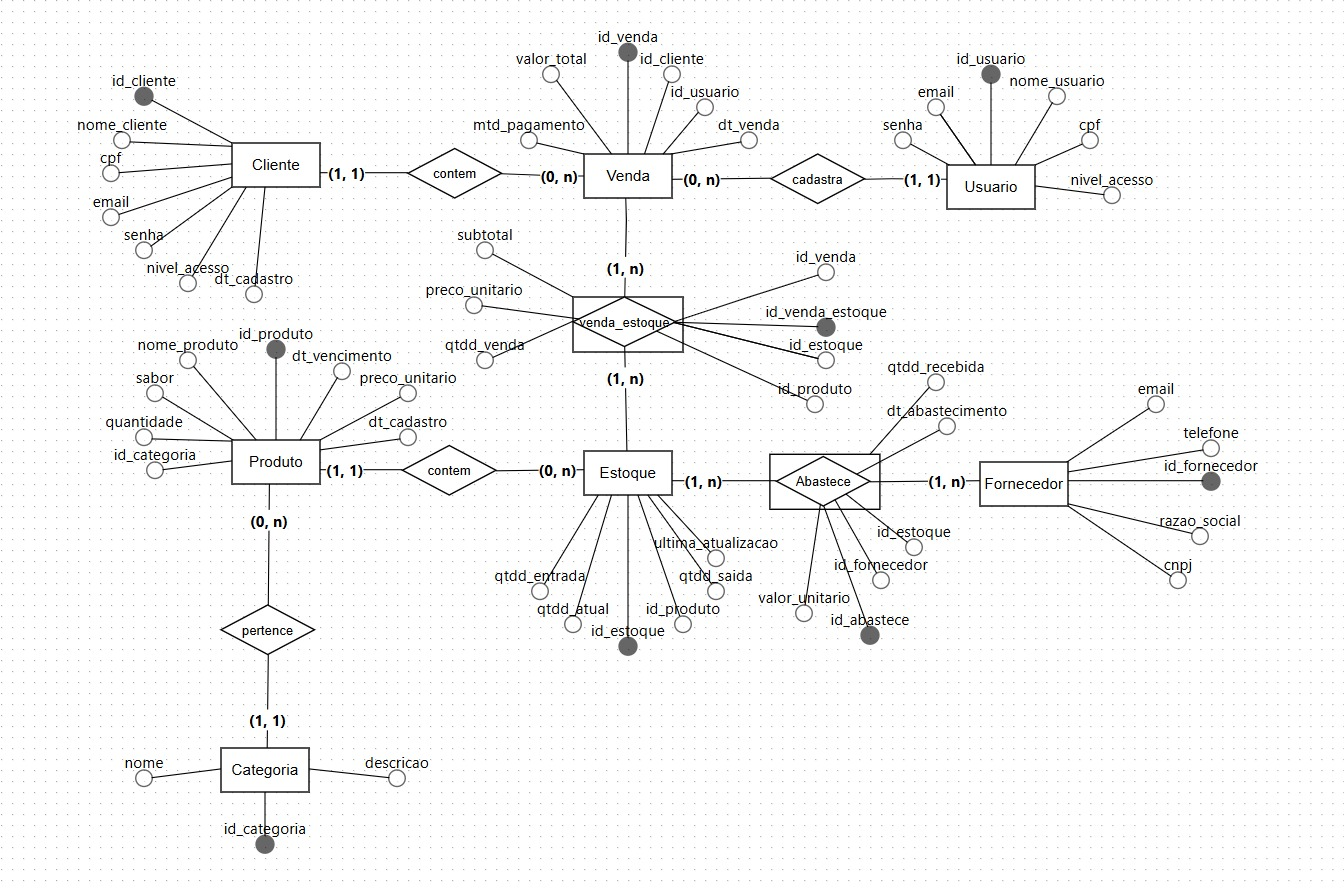
\includegraphics[width=0.7\textwidth]{documentacao/LaTex/Capítulos/img/Desenvolvimento do Projeto/Banco_de_Dados/modeloConceitual.jpg}
    \caption{Modelo Entidade-Relacionamento (MER)}
    \label{fig:mer-tropicalmix}
    \fonte{Elaborado pelos autores.}
\end{figure}

\subsection{Diagrama Entidade-Relacionamento (DER)}

A Figura~\ref{fig:der-tropicalmix} apresenta o \textbf{Diagrama Entidade-Relacionamento (DER)} do sistema \textbf{Tropical Mix}.

\begin{figure}[H]
    \centering
    \resizebox{1.1\textwidth}{0.7\textheight}{
        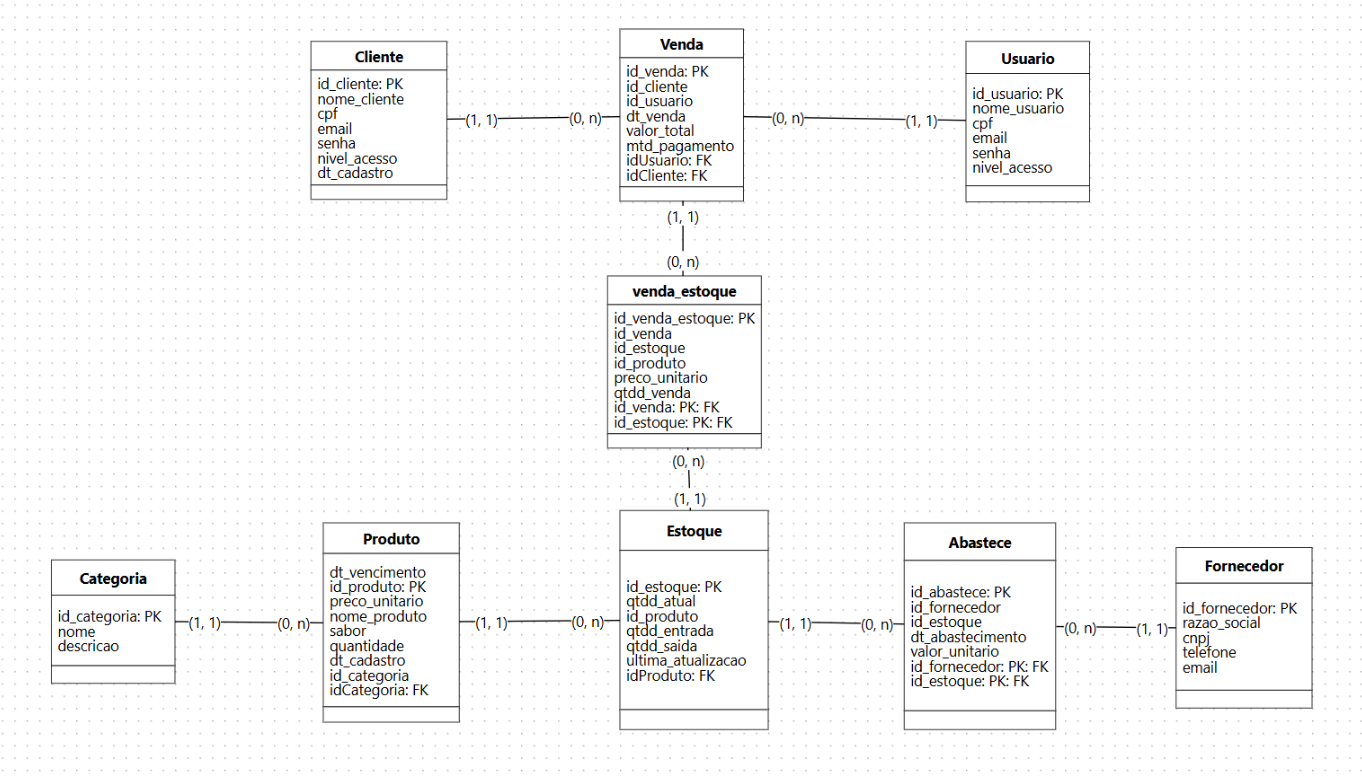
\includegraphics{documentacao/LaTex/Capítulos/img/Desenvolvimento do Projeto/Banco_de_Dados/modeloLogico.png}
    }
    \caption{Diagrama Entidade-Relacionamento (DER) do sistema.}
    \label{fig:der-tropicalmix}
    \fonte{Elaborado pelos autores.}
\end{figure}
